\documentclass[conference]{IEEEtran}
\usepackage{graphicx}
\usepackage{tikz}
 
\usepackage[colorlinks = true, citecolor = blue]{hyperref}

% math lib
\usepackage{amsmath}
\usepackage{mathrsfs}

% operators
\DeclareMathOperator*{\argmax}{arg\,max}
\DeclareMathOperator*{\argmin}{arg\,min}
\newcommand\ceiling[1]{\left\lceil #1 \right\rceil}

% empty set
\usepackage{amssymb}
\let\emptyset=\varnothing

% algorithms
\usepackage{algorithm}
\usepackage{algorithmic}
\renewcommand{\algorithmicrequire}{\textbf{Input:}}
\renewcommand{\algorithmicensure}{\textbf{Output:}}

\begin{document}
% --------------------------------------------
% --------------Change HERE! -----------------
% --------------------------------------------
\def\authorone{Eshaq Jamdar}
\def\authortwo{Martin Bojinov}
\def\groupid{4}
% --------------------------------------------
\title{CS258 Final Report: The RSA Problem}
\author{
    \IEEEauthorblockN{\authorone\ and \authortwo}
    \IEEEauthorblockA{
        Group \groupid
    }    
}

\maketitle
\IEEEpeerreviewmaketitle

% ---------------------------------------------------------------------------------------------
\section{Methods: RL-based Routing}
\subsection{RL Algorithms}
% List RL algorithms and give a brief explanation of each
\textbf{Proximal Policy Optimization (PPO)}, as described by Schulman et al. \cite{06347}, is a reinforcement learning algorithm that is classified as a gradient based reinforcement method, which means to maximize reward for an agent based on policy $\pi$. In addition to the baseline maximization of reward, \cite{06347} goes on to describe a surrogate objective function that assists with communicating to the agent how to improve policy while not deviating too far away from the original. The function 

\begin{equation}
    L^{CLIP}(\theta) = \mathbb{E}_t \left[ \min\left( r_t(\theta) A_t, \text{clip}\left(r_t(\theta), 1-\epsilon, 1+\epsilon\right) A_t \right) \right].
    \label{eq:ppo_clip}
\end{equation}
where,
\begin{itemize}
    \item $L^{CLIP}$: clipped surrogate function
    \item $\mathbb{E}_t$: expectation averaging out all possible decisions that could influence the policy
    \item $r_t(\theta)$: probability of the current policy compared to the previous
    \item $A_t$: estimator to determine the benefit of a certain action
    \item $\epsilon$: controls if policy change should occur
    \item $clip$: clip function that limits the influence of new policies via the use of epsilon
\end{itemize}

aims to make sure that stable learning is occurring. Within the clip function, policy changes happen incrementally, while also not radically shifting in policy via the use of epsilon. 

PPO algorithms are considered a good reinforcement learning algorithm for the RSA problem as PPO utilizes sampling and requires less direct interaction with the environment. In addition, due to PPO being policy based, this allows for learning based on current policy. 

\textbf{Deep Q Networks (DQN)} as described by Mnih \cite{14236}, is a reinforcement learning algorithm, that expands upon Q learning, that aims to learn good policies from high sensory inputs. In the context of this paper, sensory inputs were obtained from Atari 2600 games. Due to these games having large state spaces, the DQN algorithm developed by the authors can handle itself when encountering a large state space. 

As mentioned above, \cite{14236} builds upon Q Learning and uses this to help the agent learn good policy from bad. Actions in DQN aim to maximize future rewards over time and must determine the best course of action via the following function
\begin{equation}
    Q^*(s, a) = \max_\pi \mathbb{E} \left[r_t + \gamma r_{t+1} + \gamma^2 r_{t+2} + \ldots \mid s_t = s, a_t = a, \pi \right]
    \label{eq:dqn_clip}
\end{equation}
where,
\begin{itemize}
    \item $Q^*(s, a)$: optimal action function that returns the best possible reward after performing sequence s with action a
    \item $\max_\pi$: maximize all possible decisions
    \item $\mathbb{E}$: expectation averaging out all possible decisions that could influence the policy
    \item $r_t$: rewards based on every t episodes
    \item $\gamma$: dilute value to prioritize immediate rewards as opposed to finding a bigger reward later on
    \item $s_t$: state at time t
    \item $a_t$: action at time t
    
\end{itemize}

is the basis of Q learning and DQN uses this equation as a way to learn the best possible policy that returns the best future reward possible. 

Though this paper used Atari games as the vessel to demonstrate the use of DQN, networks, and their dynamic environments, present a perfect application of the DQN model. In addition, due to DQN's ability to replay past experiences, this allows for better insight into decisions that would otherwise be overlooked in a dynamic environment like a network. 
\subsection{State Space}
% Explain state/action/reward
% Make sure you provide enough information to reconstruct results
% Check https://gymnasium.farama.org/environments/box2d/lunar_lander/ for some examples
\begin{figure} [ht]
    \centering
    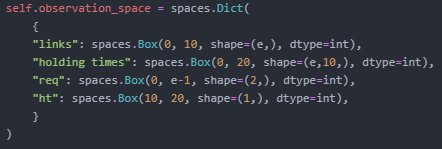
\includegraphics[width = 0.5\textwidth]{space.png}
    \caption{State Space of NetworkEnvironment}
    \label{fig:reward}
\end{figure}
The state space of the environment can be broken down as
\begin{itemize}
    \item links: represents the state of the link utilization on the network. Each link has a capacity of 10 and a total number of 15 edges (in the case of nsfnet). Shape of this would be a list of e edges.
    \item holding time: total amount of time a request occupies any link on the network. 20 is the max ht that can be accommodated. Shape here is the total number of utilization of all links on each edge.
    \item req: represents network requests. A request is defined by the first edge on the graph all the way to the last edge as the highest possible request. The shape here is [src, dst], where both contain the node information.
    \item ht: representing the random hold time for each request.
    
\end{itemize}
\subsection{Action Space}
The action space for this problem is defined as the number of shortest paths from the source node to the destination node. This action space is determined via the use of the networkx method, \texttt{shortest\_simplest\_path}.
\subsection{Reward Function}
The reward function is as follows
\begin{itemize}
    \item +1 * length of path (if allocated)
    \item -1 for blocking
\end{itemize}

% ---------------------------------------------------------------------------------------------
\section{Method: Spectrum Allocation}
% Explain your heuristic
% If you have multiple, you can make subsections 

% If you borrow some ideas from papers, cite them with bibtex (e.g. \cite{8509143})

For spectrum allocation, we used the same greedy method as A4. Once the model has selected a path between the source and destination node, it checks all links that selects the smallest-index, continuous color band.

% ---------------------------------------------------------------------------------------------
\section{Results}
\subsection{Learning Curve}
\subsubsection{Results}
In our raylib logs we see that DQN has the highest rate of learning of the 3 models. PPO returns a higher reward than the baseline but only in scenario I. For scenario II, the values vary greatly and PPO struggles to learn.

\subsubsection{Time steps}

Comparing DQN, PPO, and baseline, we see that DQN has 10k time steps at 1k intervals, while PPO and baseline have 40k time steps at 4k intervals. We can conclude that DQN learns at a more aggressive rate than PPO and baseline.

\subsubsection{Scenario II PPO vs Baseline}
In scenario II's max and mean reward, we observe that the baseline out-learns PPO. This can be seen in figures \ref{fig:max scenario 2} and \ref{fig:mean scenario 2}. We find this to be strange but attribute it to an error we had with scenario II's action space. We constantly redefine the action space to be the number of paths from the source to the destination node. Because this number fluctuates in scenario II, we ran into an error where the models will sometimes select an invalid action. To remedy this, when an invalid actions is selected, it instead blocks and receive negative reward. We explore how this can be remedied in Future Work.

\begin{figure} [ht]
    \centering
    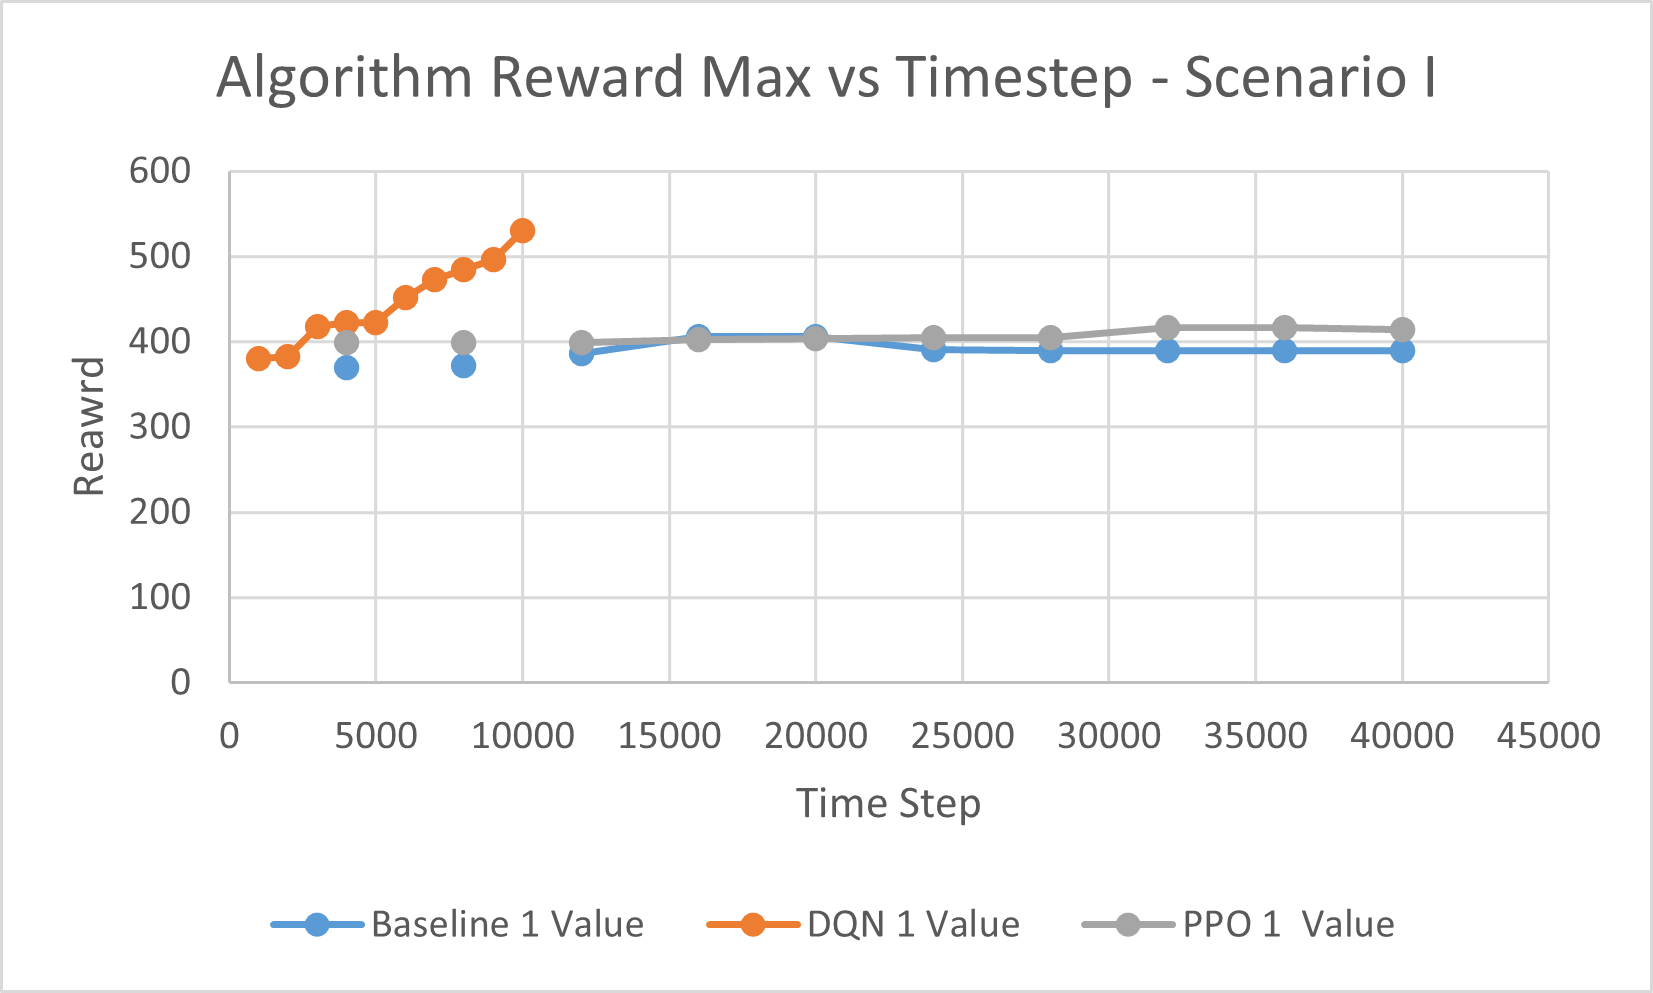
\includegraphics[width = 0.5\textwidth]{Scenario 1 Max Reward.png}
    \caption{Max learning of 3 RL models under scenario I.}
    \label{fig:max scenario 1}
\end{figure}

\begin{figure} [ht]
    \centering
    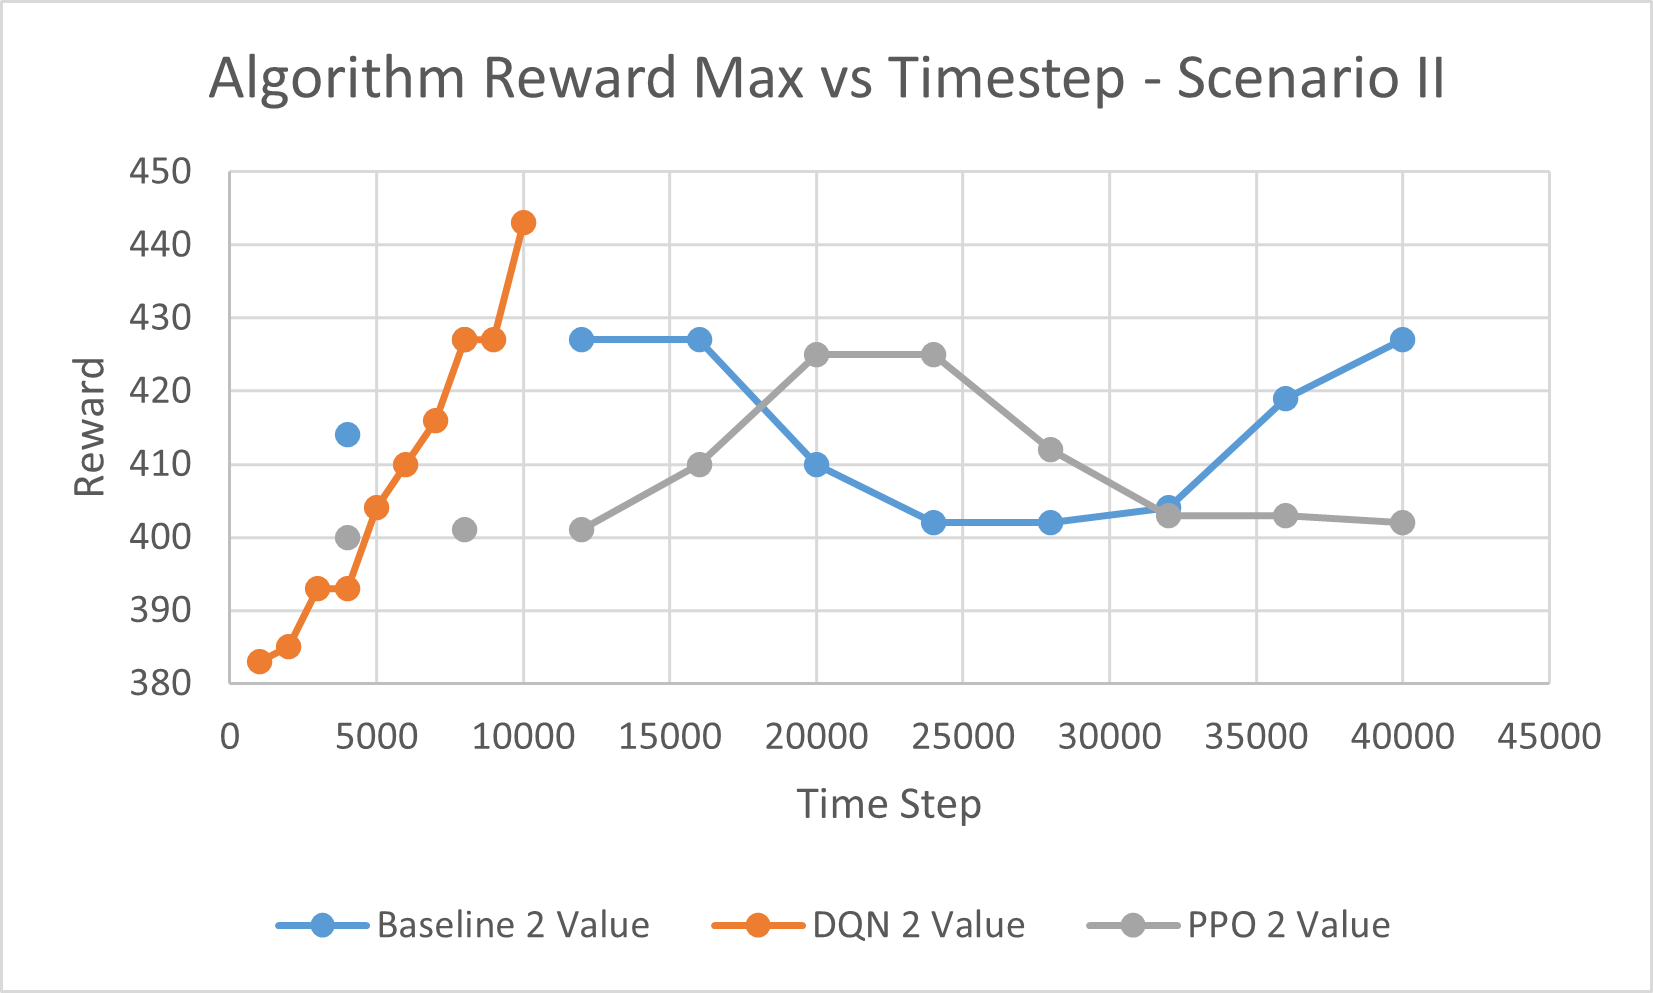
\includegraphics[width = 0.5\textwidth]{Scenario 2 Max Reward.png}
    \caption{Max learning of 3 RL models under scenario II.}
    \label{fig:max scenario 2}
\end{figure}

\begin{figure} [ht]
    \centering
    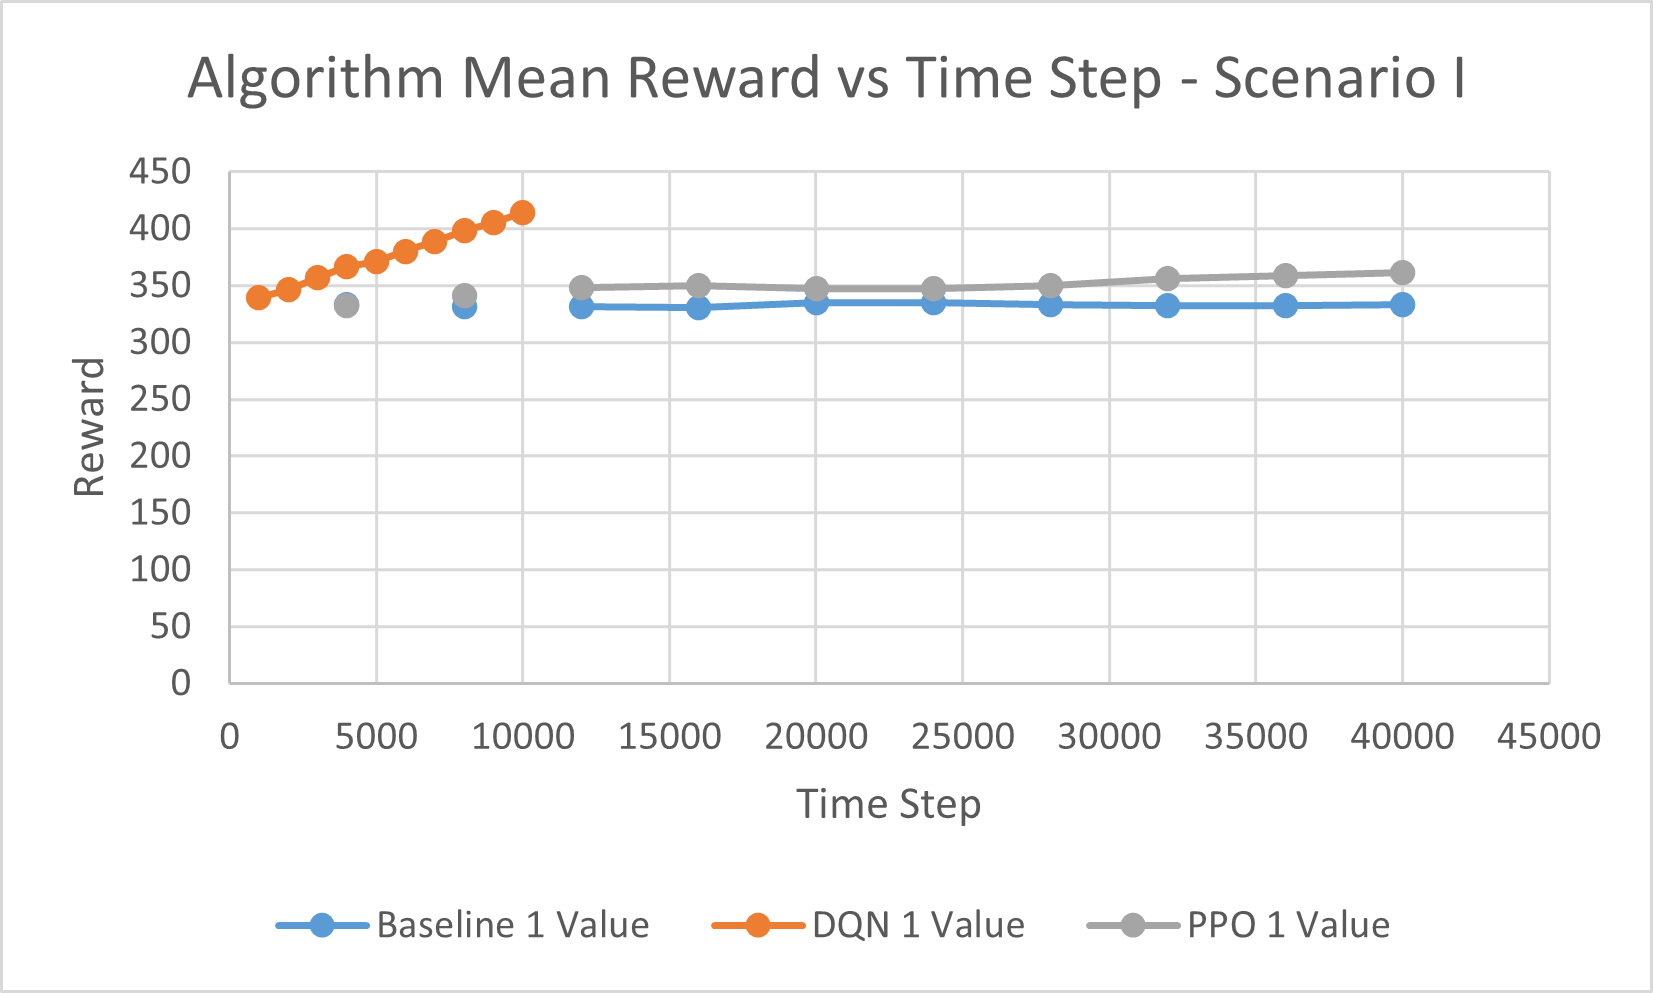
\includegraphics[width = 0.5\textwidth]{Scenario 1 Mean Reward.png}
    \caption{Mean learning of 3 RL models under scenario I.}
    \label{fig:mean scenario 1}
\end{figure}

\begin{figure} [ht]
    \centering
    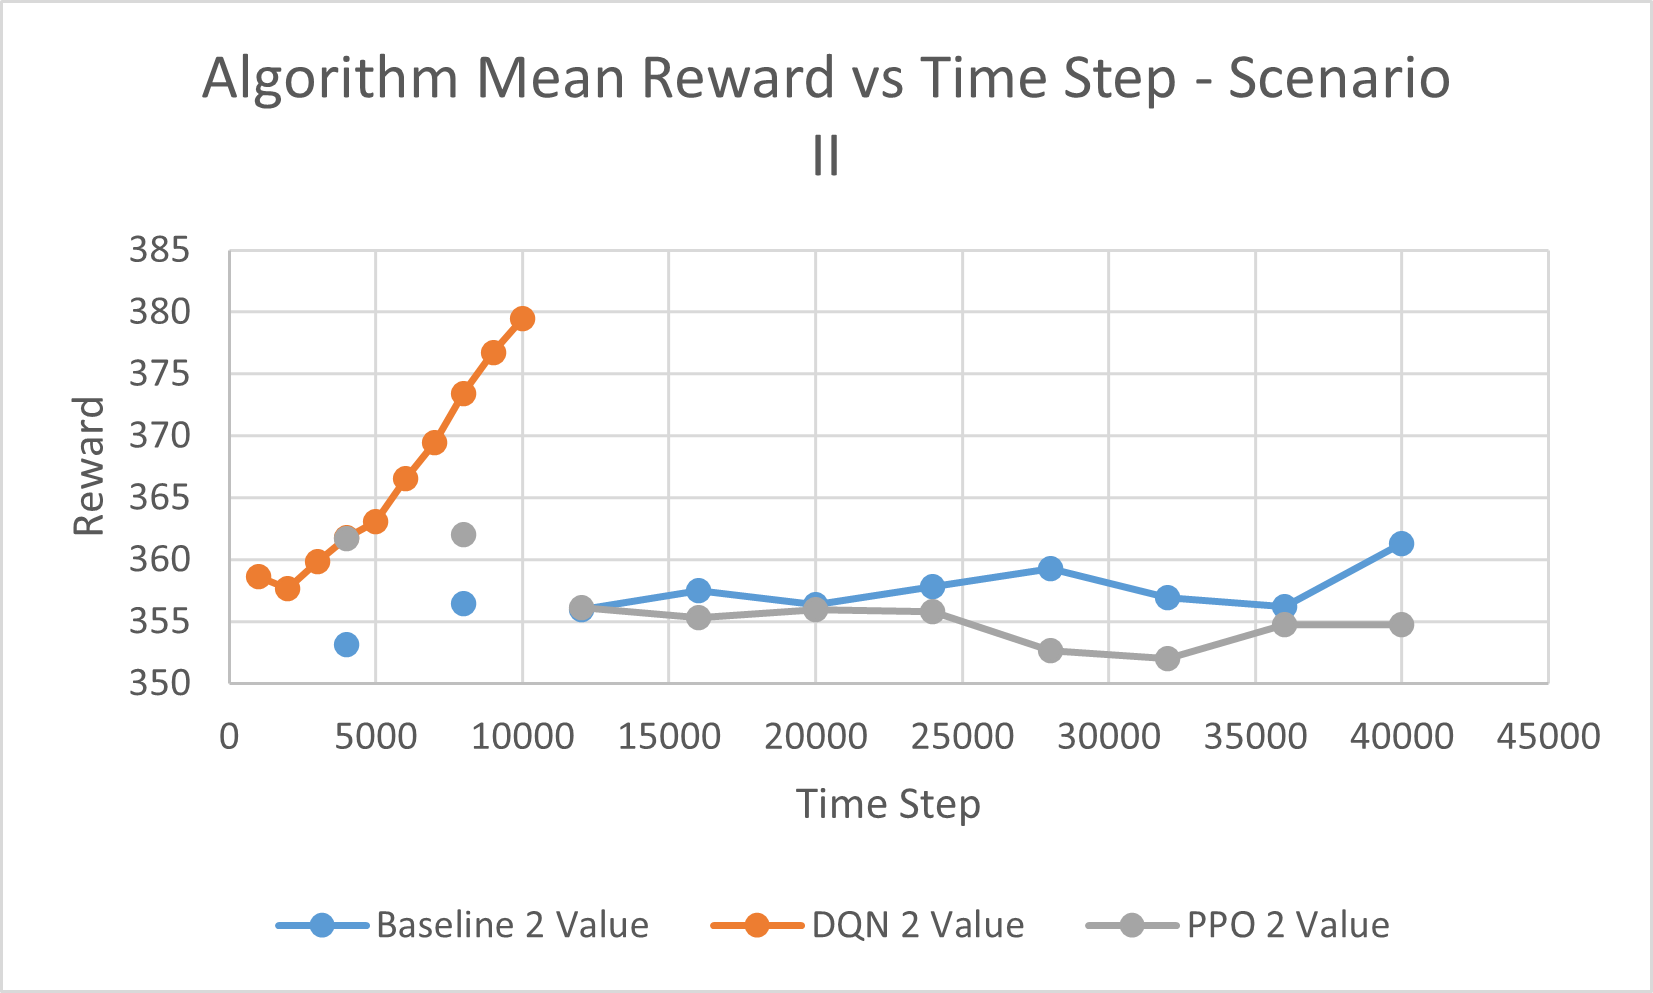
\includegraphics[width = 0.5\textwidth]{Scenario 2 Mean Reward.png}
    \caption{Mean learning of 3 RL models under scenario II.}
    \label{fig:mean scenario 2}
\end{figure}

% Insert figures
% Explain the results

\subsection{Utilization (The Objective)}

\subsubsection{Scenario I}

For this simulation, the source node is the "San Diego Supercomputer Center" and the destination is the "Jon Von Neumann Center, Princeton, NJ." Our hold time per each request is 10-20 time steps per request (which is randomly chosen). Our simple simulation using A4 (shortest distance, greedy color selection) utilizes the same links over again. As a result, these links see high utilization but the rest of the network remains empty, yielding low total network utilization. This can be seen as the bottom line of fig \ref{fig:util scenario 1}.

\begin{figure} [ht]
    \centering
    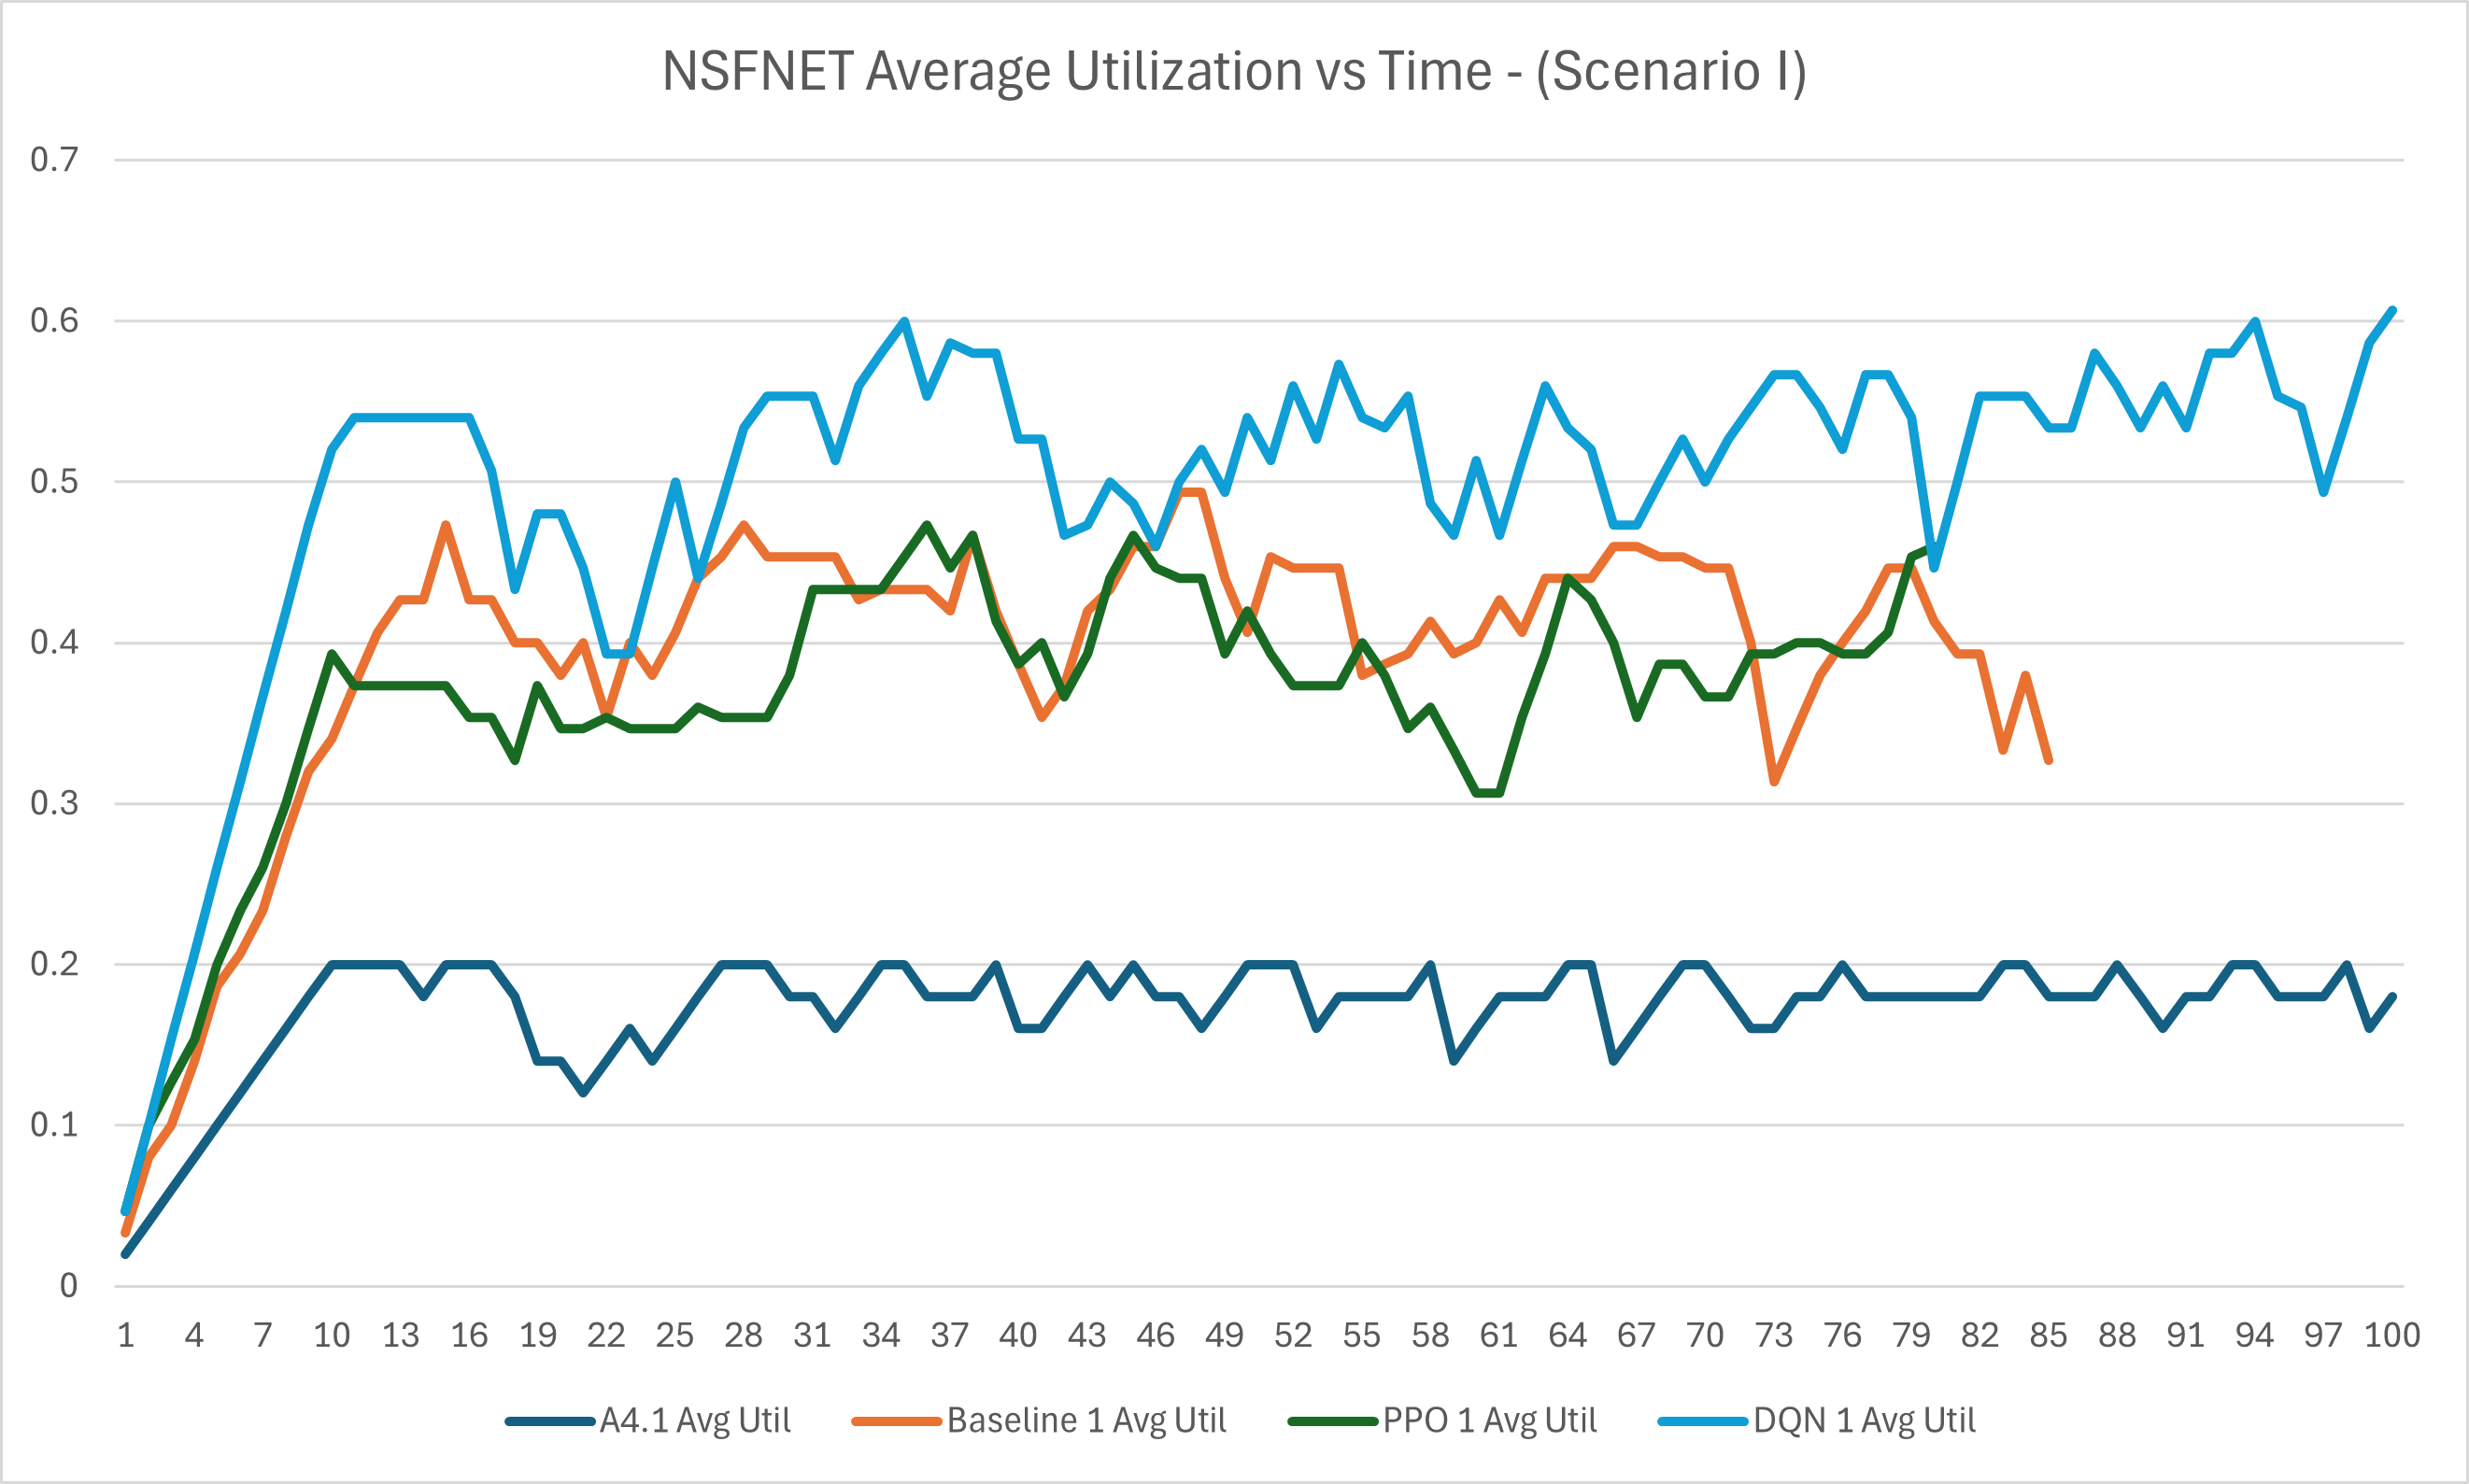
\includegraphics[width = 0.5\textwidth]{Scenario 1 Util.png}
    \caption{Average network utilization simulations of our 4 models under scenario I.}
    \label{fig:util scenario 1}
\end{figure}

\subsubsection{Scenario I - Comparison}
All three of the reinforcement learning algorithms improve upon A4. This is because, in our environment, we define the action space to be all simple paths from our source node to our destination node. Initially, they all select from these short paths at random but with time, they learn which paths yield the highest reward. A higher network utilization is achieved because more paths are considered than just the shortest path. 

When comparing the different reinforcement learning algorithms, DQN performs the best among all of the algorithms with a peak network utilization of 60\%. Our baseline and PPO models perform comparably, averaging around 45\% network utilization with PPO only marginally outperforming. In our simulations, PPO and baseline both terminated early, shortening the number of time steps the simulation ran for. 


\subsubsection{Scenario II}
In this scenario, the source and destination nodes are chosen at random. Our holding time still remains the same at 10-20 time steps per request. The shortest distance, greedy coloring algorithm of A4 performs slightly better compared to Scenario I because every link has a chance to be utilized. However, the link utilization fills up less than before, and as a result, yields a more broadly used network with a lighter load across all links.

\begin{figure} [ht]
    \centering
    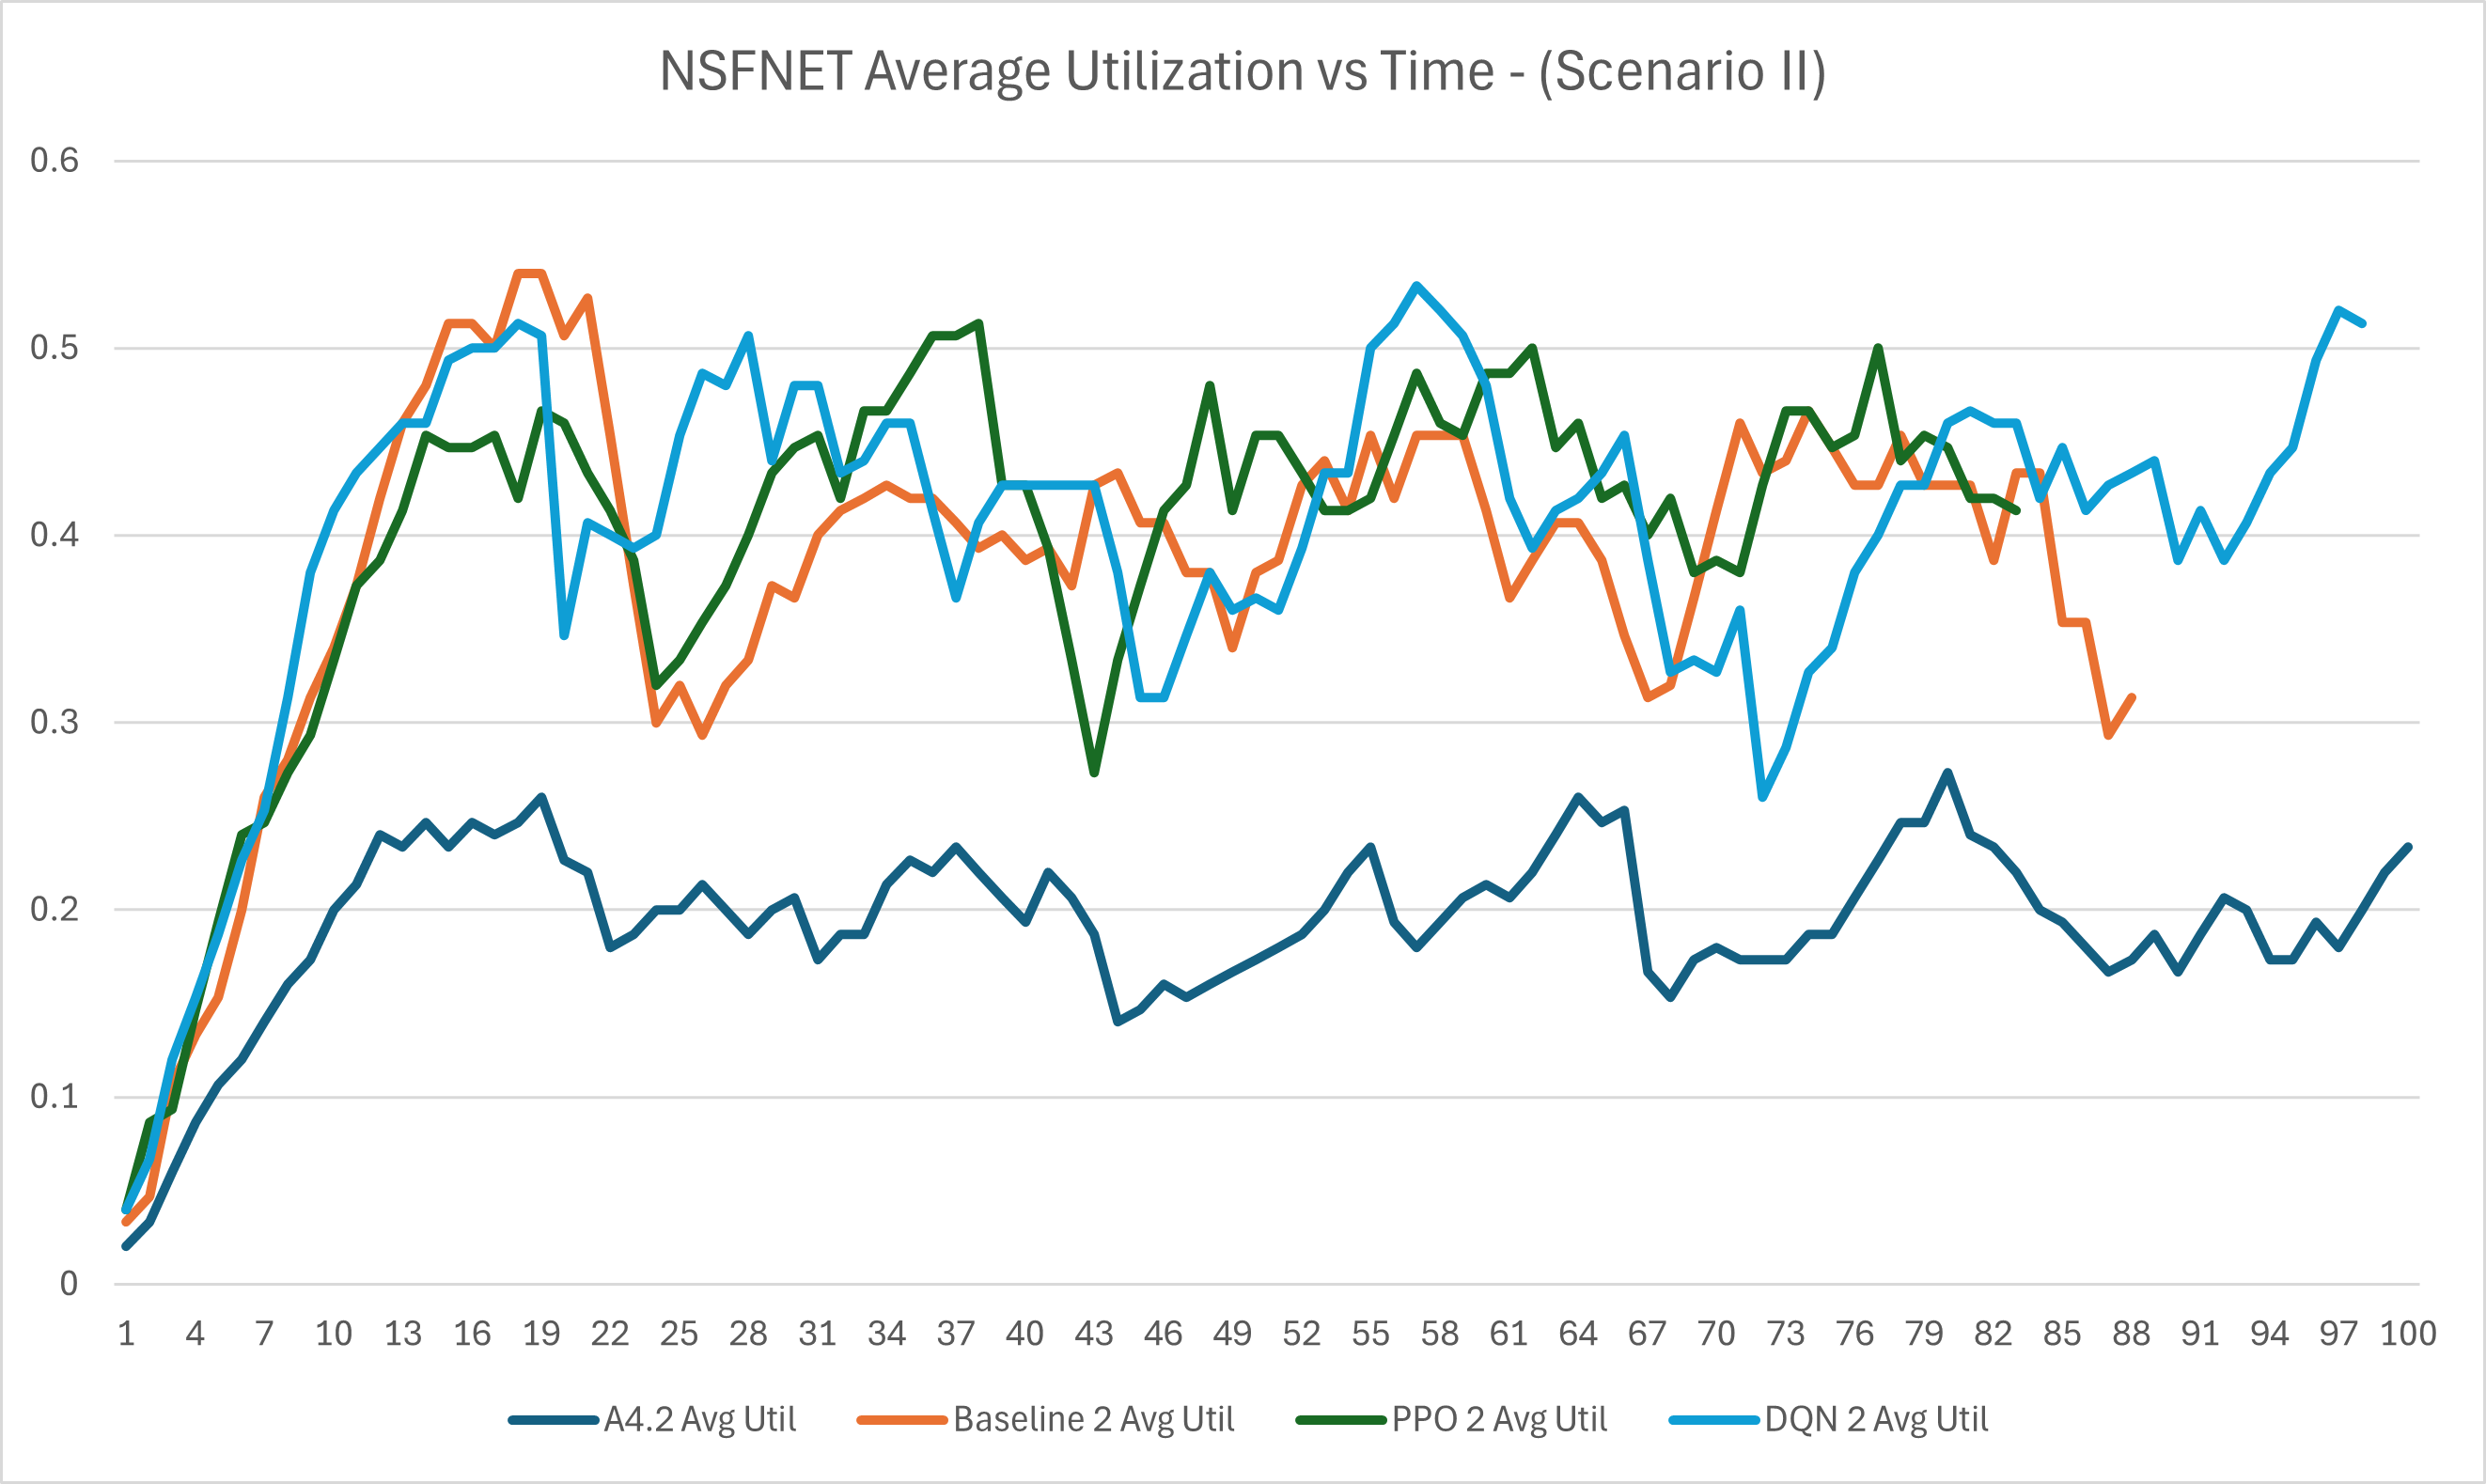
\includegraphics[width = 0.5\textwidth]{Scenario 2 Util.png}
    \caption{Average network utilization simulations of our 4 models under scenario II.}
    \label{fig:util scenario 2}
\end{figure}

\subsubsection{Scenario II - Comparison}
All three reinforcement algorithms improve upon the baseline A4 implementation. As seen in fig \ref{fig:util scenario 2}, DQN, PPO, and our baseline all fluctuate between 30\% and 50\% total network utilization. 

An interesting common behavior seen with PPO, baseline, and DQN is that all three algorithms see a rapid increase in utilization at the beginning. Despite this commonality, each algorithm has their own interesting behaviors that are indicative of their nature. When observing PPOs performance, we can see that the average utilization tends to be stable and this is indicative of PPO's ability to not shift too radically in policy overtime. However, DQN tends to have higher peaks of utilization but fails to maintain this average utilization over a longer period of time. Thus behavior can be attributed towards the Q learning and exploring many different policies until the highest reward can be located. 

Within the data, PPO and baseline mysteriously terminate the simulation in under 100 time steps. As of now, it cannot be determined why this behavior exists and further debugging and running of the simulations is required to better understand this issue.


% ---------------------------------------------------------------------------------------------
\section{Conclusion}

In our experiments, we have three RL models that outperform our simple A4 method. DQN and PPO are made to learn. Meanwhile baseline does not learn and serves as a reference point. Across all metrics, DQN performs the best. PPO slightly outperforms baseline in scenario I but runs into issues in scenario II.

\subsection{Future Work}

While the results were substantial, they could be improved upon. First, it would be important to figure out why PPO and Baseline both terminate early. Being able to solve this problem would improve our data to be more uniform. 

Secondly, we ran into an issue with gymnasium regarding our action space. We set the action space to be the number of possible paths from source node to destination node. This works great for scenario I as it is a fixed amount. For scenario II, this number fluctuates. Despite updating the action space at each step, the environment will sometimes pass invalid action values. In this case, we have to block and pass a negative reward, incorrectly punishing the model. In the future we can fix this with "action masking" \cite{action_mask_tutorial}\cite{action_mask_stack_overflow}. Alternatively, we can redefine our action space to be bound by the smallest number of paths between all nodes. In the case of NSFNET, this would be 1.

Finally, in our reward function, we reward the model based on how many links it utilizes in a path. This in turn rewards longer paths and raised network utilization. In the future, it would be interesting to experiment with different rewards. For example, rewarding paths that are currently under-utilized or paths that maximize total network utilization.





\bibliography{ref}
\bibliographystyle{ieeetr}


\end{document}



